\chapter{Lezione 1}
\href{https://sites.google.com/site/compilerclassunitn/}{Vecchio sito}

Riguardo linguaggi di analisi lessicale, si usano \textbf{simboli e caratteri}. Ho una tavola dei simboli creata in base al programma
(e al compilatore). Restituisce un \textbf{token} (puntatore) ad un record nella tavola dei simboli.
La maggior parte delle implementazioni usano un numero come \textbf{identificatore}.
Analisi sintattica si basa sulla grammatica del linguaggio.
Grammatica generativa vedere se \'e possibile generare una frase con la grammatica (syntax error).
abstract syntax tree; nelle grammatiche formali metto in evidenza l'assegnamento. 

$a = b + c \cdot 60$

\Tree [.= $a$ [.+ $b$ [.* $c$ $60$ ] ] ]
\Tree [.assegnamento $id_1$ [.+ $id_2$ [.* $id_3$ $id_4$ ] ] ]

L'analisi semantica si occupa di vedere se c'\'e una corretta semantica (variabili dichiarate precedentemente). Se * necessita di un 
float allora 60 dev'essere convertito a float 

\begin{center}
\Tree [.* {\ldots} [.{intToReal(num)} 60.0 ] ]\\[5pt]
\end{center}

Generazione di codice intermedio: 
\begin{tabular}{ll|l}
$temp_1$ =& intToReal(60) & \\
$temp_2$ =& $id_3 * temp1$ & VISITA DELL'ALBERO\\
$temp_3$ =& $id_2 + temp2$ & \\
$id_1$ =& $temp_3$ & \\
\end{tabular}\\[5pt]

\Tree [.D [.\fbox{Codice intermedio} $M1$ $M2$ $M3$ ] ]\\[5pt]

Una \textbf{grammatica} \'e una tupla G(V, T, S, P) con:
\begin{tabular}{ll}
V & vocabolario\\
T & set simboli terminali\\
S & start symbol\\
P & set delle produzioni\\
V$\backslash$T & simboli\\
$\epsilon$ & parola vuota, non pu\'o essere un terminale!\\
%[Sono tutti insiemi!] & \\
\end{tabular}\\[5pt]

\begin{tcolorbox}\begin{center}
Per convenzione i caratteri in maiuscolo denotano simboli non terminali mentre in minuscolo terminali. Quindi i simboli in T sono 
tutti lettere minuscole.
\end{center}\end{tcolorbox}

Considero X, Y variabili, generico simbolo in V e $\alpha\ \beta\ \delta\ \text{stringe su } V^*$ (ripetere 0+ volte i simboli)  
$S \rightarrow aSb,\ S\rightarrow \epsilon,\ S \rightarrow A$, T=a, b non terminali ($V\backslash T$) = S, A 

Lo start symbol \'e usato nella prima produzione solo se produzioni libere dal contesto.
Produzione legittima $aS\rightarrow b$ S a destra di una P non libera dal contesto.

Una grammatica generata \'e libera dal contesto (context free) se $\forall$ sua produzione ha la forma: $A\rightarrow \beta$ con A 
simbolo non terminale. ($\alpha \rightarrow \beta$, $\alpha$ deve contenere simboli non terminali).

$S \rightarrow ASb|\epsilon,\quad S\rightarrow \epsilon$ (privo di derivazione)

$S \rightarrow aSb \rightarrow ab$
$S \rightarrow aSb \rightarrow aaSbb \rightarrow aabb \implies \{a^nb^n\ / \ n \geq 0 \} $ Struttura di bilanciamento per parentesi (blocchi begin end).

$\mu = \mu_1 \alpha \mu2,\ \alpha \rightarrow \beta$ \'e produzione di grammatica G e $\gamma$ \'e uguale a $\mu_1 \beta \mu_2$
derivazione in pi\'u passi $\mu$ deriva in uno o pi\'u passi data la grammatica G se ho una sequenza L(G) linguaggio generato da grammatica = insieme di stringhe

$S \rightarrow aSb,\ S \rightarrow aAb,\ S \rightarrow ab,\ A \rightarrow aaAb,\ A \rightarrow \epsilon$
$\{w \ / \ w \in T^* \land s \implies^+ W\}$
$\{ a^n b^n| n > 0,\ S = 0,\ S = 1 \}$
L = $\{a^n b^n \ / \ n > 0\}$

Dato il linguaggio L possono esistere pi\'u grammatiche diverse tra loro che generano L \'e indecidibile il linguaggio generato dalla 
grammatica G, $\not\exists alga dato G e dato a L che dice che L = L(G)$.

$S \rightarrow aSBc|abc$
$cB \rightarrow Bc$
$bB \rightarrow bb$


$S \rightarrow AB$
$A \rightarrow A$
$A \rightarrow a$
$B \rightarrow Bb$
$B\rightarrow b$
tutto ci\'o che deriva da A \'e indipendente da ci\'o che deriva da B.
aaa Ab b
aaa aaAb bb
$a^5$ aaAb $b^3$
${a^{2n+1}b^{n+1},\ n \geq 0}$

$S \rightarrow aB$, $S\rightarrow  \epsilon$, $L(G) = \not 0$, $L(G) = \{ \epsilon \}$,
 $S \rightarrow 0B|1A $, $A \rightarrow 0|0S|1AA$, $B\rightarrow 1|1S|0BB$

Definisco $G_1 \ / \ $ il linguagigo L generato da $G_1 = $ insieme delle parole $L(G) = \{ a^k b^N, k > 0 \}$
$S \rightarrow ab|aS|Sb$ $S \rightarrow aS|aB$ $B \rightarrow bB|b$, $S\rightarrow^+ a^iS$

$S\rightarrow AB,\ A \rightarrow Aa|a,\ B \rightarrow bB|b$

$L(G) = \{a^ib^mc^{2n}\}$

$S\rightarrow AB,\ A \rightarrow Aa|a,\ B \rightarrow bBcc|bcc$

$a^kb^nd^2k,\ S\rightarrow Sdd|aBdd,\ B\rightarrow bB|b,\ S\rightarrow aSdd|abdd$

non terminale $\alpha \rightarrow \beta$ stringa 
    grammatiche dipendenti dal contesto per vedere la differenza fra context dependent e quelle libere. Grammatiche libere si prestano in modo 
naturale a descrivere derivazioni in viste ad albero.

$S \rightarrow aSb|ab$
abstract syntax tree da albero di derivazione\Tree [.S a [.S a b ] b ] aabb, derivazione canonica $\mu \rightarrow \gamma$
Ambiguit\'a di G 
Nel caso di grammatiche libere si definiscono derivazioni canoniche destre e sinistre (rightmost/leftmost derivating)
nel caso di rightmost si richiede che ad ogni passo di derivazione ($\mu \rightarrow \gamma$) venga rimpiazzato il terminale 
t a destra in $\mu$ (rispettivamente leftmost $\rho$ a sinistra).

G \'e ambigua se $\exists\ L(G) \ / $ esistono per w due derivazioni canoniche distinte entrambe destre o entrambe sinistre.
$E \rightarrow E+E|E*E|+$ (il + associa a sinistra)
\Tree [.E [.E [.E + ] + [.E + ] ] + [.E + ] ]
\Tree [.E [.E + ] + [.E [.E + ] + [.E + ] ] ]   
[Analogo con il *]

$S \rightarrow if\ b\ then\ S\ |\ if\ b\ then\ S\ else\ S\ |\ altro$
$if\ b\ then\ if\ b\ then\ altro\ else\ altro$
$if\ b\ then\ S\ else\ S$

G(V, T, S, P) 
Un linguaggio L \'e libero (da contesto) se esiste una grammatica libera G tale che L = L(G).
In generale dato un linguaggio generale L ed una grammatica G $\not\exists$ un algoritmo per dimostrare che L = L(G)

Grammatiche libere
chiusura (se faccio operazioni su stringhe restano grammatiche libere)

Lemma: La classe dei linguaggi liberi \'e chiusa rispetto all'unione. 
Il linguaggio che contiene tutte e sole le parole $W \in L_1\cup L_2$ \'e esso stesso un linguaggio libero.

$L_1$ \'e libero $\implies \exists\ G_1 = (V_1,T_1,  S_1, P_1) \ / \ L_1=L(G_1) $ [analogo per $L_2$]

avendo ridenominati i non-terminali di $G_1$ e $G_2$ in modo da non avere anonimia

Lemma: La classe dei linguaggi liberi \'e chiusa rispetto alla concatenazione (se $L_1,\ L_2$ sono liberi allora 
$\{ v_1v_2 \ / \ v_1 \in L_1 \land v_2 \in L_2 \}$ \'e un linguaggio libero).

G=(V,T,S,P) $\alpha \rightarrow \beta,\ \alpha ,\ \beta \in B^+ $ con al meno un terminale
In una grammatica libera $A\ (non terminale)\rightarrow \beta$ Le grammatiche libere sono quelle in cui tutte le produzioni in P hanno tutte 
forma $A \rightarrow \beta$.

Un linguaggio \'e libero se $\exists$ una grammaica libera che lo generale

ie) linguaggio $\{ a^nb^n\ / \ n > 0 \}$ libero perch\'e $\exists$ una grammatica libera che lo genera ($G_1$).
$G_1\qquad S\rightarrow aSb/ab$ $G_1$ libera
$G_2\qquad s\rightarrow aAb,\ A\rightarrow aaAb,\ A\rightarrow \epsilon$ $G_2$ non libera
$\Box$   

$L=\{ vw\ / \ w \in \{ a,b\}^* \}$ 
Con il \textbf{pumping lemma} posso dimostrare se un linguaggio \'e libero o meno.

Pumping lemma: Sia L un linguaggio libero allora $\exists\ p\in \mathbb{N}^+ \ / \ \forall\ z\in L:\ |z|>p\ \exists\ uvwxy \ / \ z = uvwxy 
\land |vwx| \leq p \land |vx|>0 \land\ \forall\ i \in \mathbb{N} uv^iwx^iy \in L$.
\begin{tabular}{ll}
$\exists\ p\in \mathbb{N}^+$ & esiste una costante $p>0$\\
$\forall\ z\in L:\ |z|>p$ & ogni parola con pi\'u elementi di p\\
$\exists\ uvwxy \ / \ z = uvwxy $ & esistono 5 sottostringhe che compongono z\\
$|vwx| \leq p$ & la lunghezza delle 3 stringhe centrali \'e minore di p\\
$|vx|>0$ & la seconda e la quarta non sono mai entrambe nulle\\
$\forall\ i \in \mathbb{N} uv^iwx^iy \in L$ & se ripeto i volte (i pu\'o essere 0) la 2 e la 4 sono ancora in L\\
\end{tabular}

G $\qquad S\rightarrow aSb|ab$
G $\qquad S\rightarrow A,\ A\rightarrow aAb|ab$

Chomsky normal form (no doppioni)

ie) 
$G_1 \qquad S \rightarrow aSb|ab|B,\ B\rightarrow aBb|ab \leftarrow$ doppioni
$G \qquad S\rightarrow A,\ A \rightarrow aAb|ab $

Dim L \'e linguaggio libero $\implies \exists$ una grammatica G in Chomsky Normal Form tale che L = L(G).
Definisco P come la lunghezza della parola pi\'u lunga che pu\'o essere derivata usando un albero di derivazione i cui cammini 
dalla radice sono lunghi al pi\'u come il numero di simboli non teminali della grammatica $(|V\backslash T|$).
\Tree [S [.$A_1$ [.$A_2$ [.\ldots [.a] ] ] ] ] 
$S \rightarrow aSb|ab$
Albero di derivazione: piglio un non terminale e lo espando con figli quanto vale $\beta$
\Tree [.S a [.S a b ] b ]
\Tree [.S a [.S a [.S a b ] b ] b ] \ldots


P \'e la lunghezza della parola pi\'u lunga che posso linitare.
$S\rightarrow A_1 \rightarrow A_2 \rightarrow ...\rightarrow A_k \rightarrow a$ [tutti simboli non terminali tranne a]


ie) p = 2, se prendo una qualunque perola pi\'u lunga di 3 generata da G, aaaabbbb la posso dividere in 5 con due pumpable
u=aa, v=a, w=abb, x=b, y=b 

Se prendo $z\in L \land |z| > p \implies $ ho dovuto usare un albero di derivazione $\ / \ \exists $ al meno un cammino pi\'u lungo 
di $|V\backslash T|$ per definizione di z.
$\implies $ ho un non terminale ripetuto al meno due volte 
$\implies \exists$ al meno un non terminale che occorre al nomo 2 volte lungo quel cammino

con l'un-pumping la parola sta sempre nel linguaggio (taglio un pezzo di albero) 
ie)
\Tree[.S a [.S a [.S a b ] b ] b ]

\begin{center}
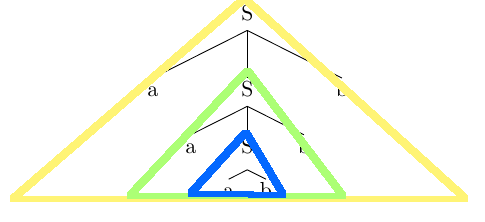
\includegraphics[scale=0.4]{Chapters/Img/c01_01.png}
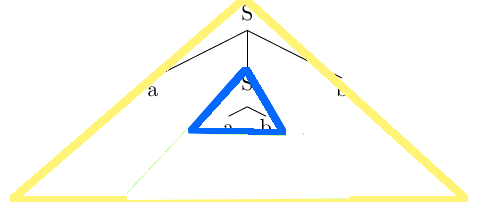
\includegraphics[scale=0.4]{Chapters/Img/c01_02.png}\\
\end{center}

$\Box$

Dato che w e x non possono essere entrambi nulli al massimo avr\'o  $A \rightarrow aA,\ o\ A \rightarrow Aa$

\begin{center}
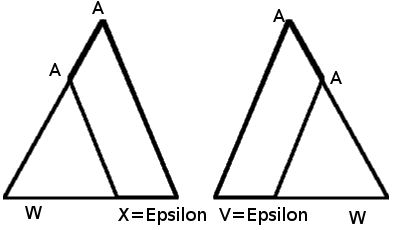
\includegraphics[scale=0.4]{Chapters/Img/c01_03.png}
\end{center}

ie) linguaggio libero $\{a,b\},\ S \rightarrow ab$ 
\begin{center}
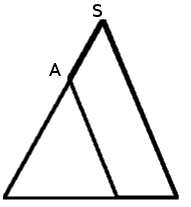
\includegraphics[scale=0.4]{Chapters/Img/c01_04.png}
\end{center}

\section{Uso del Pumping Lemma per determinare linguaggi liberi}
Tesi: Sia L un linguaggio libero allora 
$\exists p \in \mathbb{N}^+\ / \ \forall\ z \in L:|z|>p\ \exists\ uvwxy \ / \ (z = uvwxy \land |vwx| \leq p \land |vx| > 0 \land \forall\ i \in \mathbb{N} uv^iwx^iy \in L)$

Considero $L_1=ww\ / \ w \in \{a,b\}^*$ non \'e libero

Dim: Suppongo $L_1$ libero, sia p un numero naturale positivo qualunque (se scelgo un p arbitrario la dim non serve a nulla).
Sia $z=a^pb^pa^pb^p$ allora $z \in L_1,\ |x| > p$. Siano $uvwxy\ / \ z = uvwxy \land |vwx| \leq p \land |vx| > 0$, distinguiamo varie possibilit\'a:
\begin{itemize}
\item[1)] vwx \'e composto da \lq a \rq\ che occorrono a sinistra ($w_1$)\\
\item[2)] vwx \'e a cavallo e contiene sia \lq a \rq\ che \lq b \rq\ in $w_1$\\
\item[3)] vwx contiene solo \lq b \rq\ in $w_1$\\
\item[4)] \lq b \rq\ in $w_1$ e \lq a \rq $\in w_2$\\
\item[5,6,7)] ...speculare su $w_2$\\
\end{itemize} 

Nei casi 1, 3, 5, 7 considero le parole $z^1=uv^0wx^0y$ (i=0);
nel caso 1 sono certo di togliere alcune occorrenze di a quindi avr\'o $z^1 = a^k b^p a^p b^p,\ k < p \implies z^1 \not\in L$. 
Nel caso 3 $z^1 = a^p b^k a^p b^p,\ k < p \implies z^1 \not\in L$.
Nel caso 5 $z^1 = a^p b^p a^k b^p,\ k < p \implies z^1 \not\in L$.
Nel caso 7 $z^1 = a^p b^p a^p b^k,\ k < p \implies z^1 \not\in L$.

Nei casi 2, 4, 6 invece avr\'o ancora $ z^1=uv^0wx^0y $ (i=0);
Nel caso 2 $z^1 = a^k b^p a^p b^p,\ o\ a^p b^k a^p b^p,\ o\ a^j b^k a^p b^p,\ j,k < p \implies z^1 \not\in L$ .
...
\begin{comment}
How not to: se avessi preso $\{ww \ / \ w\in\{a,b\}^*\}$ sia $z = (ab)^p (ab)^p$, prendo p=4, $v\in\epsilon, x=a, i = 0$ cos\'i non 
dimostro niente perch\'e se voglio dimostrare con il pumping lemma la negazione della tesi devo dimostrare un asserto che vale $\forall p \in \mathbb{N}^+$.
Pertanto non posso prendere un arbitrario p=4.

ie) $\{a^nb^nc^j/n,j\geq 0\}=L_{17}$
$S \rightarrow aSb|B$
$B \rightarrow cB|\epsilon $
$acb \in L_{17}$
\Tree[.S a b [.S a b [.S $\epsilon$ ] ] ]
\Tree[.S a [.S [.B c [.B $\epsilon$ ] ] ] b ]


$S \rightarrow abA|B$
$B \rightarrow cB|\epsilon$
\Tree[.S [.A \ldots \ldots ] [B \ldots \ldots ] ]


$S \rightarrow AB$
$A \rightarrow aAB|ab|\epsilon$
$B \rightarrow Ab|c|\epsilon$
\Tree[.S [.A a [.A \epsilon] b ] [.B \epsilon ] ]
\Tree[.S [.A a b ] [.B \epsilon ] ]
\end{comment}